\section{Numerical accuracy and supporting results}\label{supp:numdetail}\label{supp:transrecords}
\subsection{Grid refinement, derivative, and solver checks}\label{supp:accuracy}
All differences here are observed numerical comparisons, not certified
bounds. Direct attribution-column differences are at most 0.178\% for
11 versus 41 states and $1.1\times10^{-4}\%$ for six-query/single-OD
41 versus 81 states. Near-zero accounts on 41/81/161 grids change by
less than $5\times10^{-6}$ percentage points (absolute $<0.01$); the
learned 201/801-state relative difference is $4.97\times10^{-6}$.
Implicit versus re-solved central-difference Jacobian errors are at most
$7.6\times10^{-5}$ (halved step $2.5\times10^{-5}$), or
$3.0\times10^{-8}$ for six-query/single-OD columns. Newton versus
successive-averages differences over 1,353 solves are at most
$1.31\times10^{-11}$. Maximum fixed-point and balance residuals are
$3.10\times10^{-8}$ and $1.82\times10^{-11}$ veh/h. Scalar completeness
relative discrepancies are at most $3.36\times10^{-5}$ for
frozen/re-routing settings and $1.9\times10^{-7}$ for single-OD checks.
Per-edge endpoint checks give relative column errors
$7.7\times10^{-8}$--$1.1\times10^{-6}$ and maximum entry residuals
$5.4\times10^{-4}$--$1.6\times10^{-2}$ TSTT units. Per-query records
remain in the arrays. The direct $(10,16)$ account change is 24.80\%
on its 41-state grid; Figure~\ref{fig:respfield} uses the seed-zero
learned model on 201 states (24.8\%).

\begin{figure}[htbp]
\centering
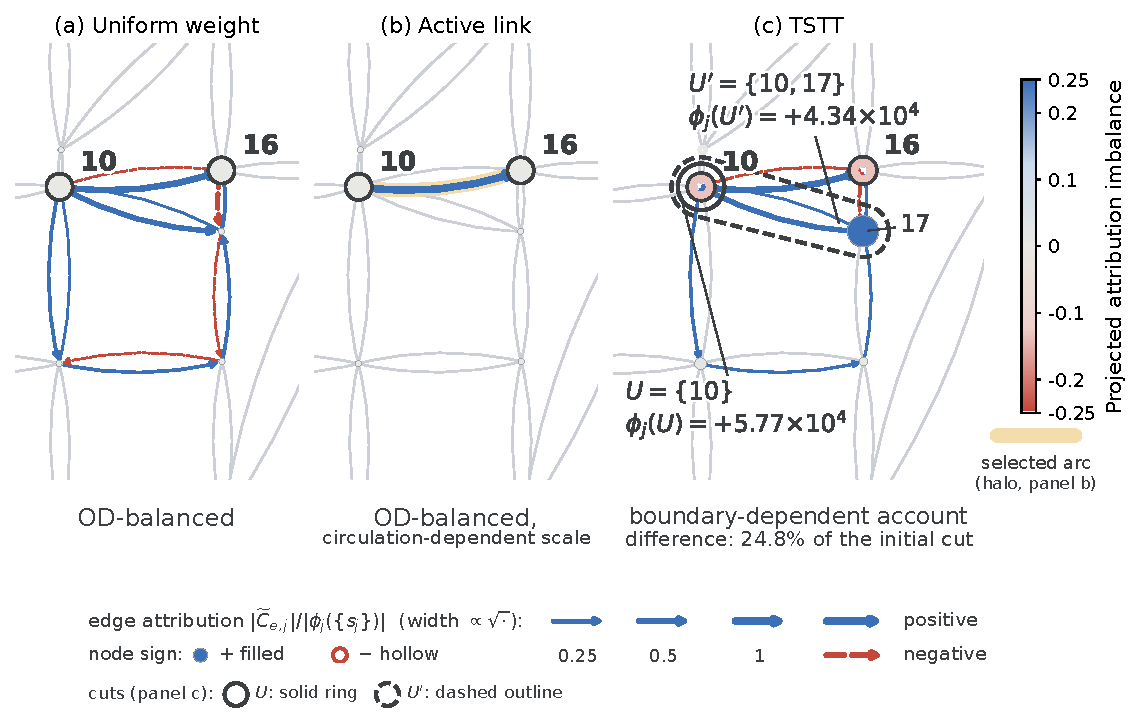
\includegraphics[width=0.84\linewidth]{../figures/fig_resp_field_v100.pdf}
\caption{OD $(10,16)$ endpoint attributions, zero background, learned
seed $0$. (a) Uniform weights give cut consistency. (b) The active-link
outcome balances in the OD direction but has no response-independent scale.
(c) The signed TSTT boundary account decreases by $24.8\%$ when the
boundary expands from $\{10\}$ to $\{10,17\}$.
Widths encode attribution magnitude; node colors show the projected
attribution imbalance $(d_j)_v$ (Eq.~\eqref{eq:endpointd}) divided by
the absolute origin-cut value.}
\label{fig:respfield}
\end{figure}

\subsection{Normalization, cancellation, and sensitivity}\label{supp:additional}
\paragraph{Complete cut-range table.}
Table~\ref{tab:cutspreadfull} completes the three representative rows of
Table~\ref{tab:cutspreadperod} with all eight study ODs.
\begin{table}[pos=htbp]
\caption{TSTT cut ranges as percentages of each account's absolute
origin-cut value, all eight study ODs (complete version of
Table~\ref{tab:cutspreadperod}). A: zero background; B: frozen background
flows; C: background demands fixed, all traffic re-equilibrated. Learned
values are five-seed medians (ranges); all SUE columns are direct
($41$ quadrature points, implicit sensitivities).}\label{tab:cutspreadfull}
\footnotesize
\begin{tabular*}{\tblwidth}{@{\extracolsep{\fill}}lccccc}
\toprule
& \multicolumn{4}{c}{Unrestricted range (\%)} & Connected (\%)\\
\cmidrule(lr){2-5}\cmidrule(lr){6-6}
OD & Learned A & SUE A & SUE B & SUE C & SUE C\\
\midrule
$(17,10)$ & $59.71$ $(58.92$--$61.23)$ & $59.95$ & $56.38$ & $54.77$ & $35.27$ \\
$(10,17)$ & $37.55$ $(37.40$--$37.94)$ & $37.48$ & $43.62$ & $49.11$ & $31.57$ \\
$(16,10)$ & $36.80$ $(36.41$--$38.40)$ & $36.86$ & $39.99$ & $166.26$ & $127.72$ \\
$(10,16)$ & $26.85$ $(26.68$--$27.07)$ & $26.94$ & $34.02$ & $109.04$ & $83.80$ \\
$(15,10)$ & $0.84$ $(0.69$--$1.16)$ & $0.77$ & $21.98$ & $84.05$ & $58.24$ \\
$(10,15)$ & $0.81$ $(0.76$--$0.88)$ & $0.77$ & $18.89$ & $71.88$ & $49.90$ \\
$(10,11)$ & $0.23$ $(0.10$--$0.35)$ & $0.0075$ & $1.17$ & $84.67$ & $51.27$ \\
$(11,10)$ & $0.18$ $(0.03$--$0.27)$ & $0.0073$ & $0.79$ & $81.09$ & $48.98$ \\
\bottomrule
\end{tabular*}
\end{table}
\paragraph{Error-metric definitions.}
The surrogate test flow error is, within each seed, the mean over the
$857$ test demands of
$\|f(q)-F^{\mathrm{SUE}}(q)\|_2/\|F^{\mathrm{SUE}}(q)\|_2$, reported
as the median over the five seeds; Jacobian column errors
$\|J_j^{\mathrm{learned}}-J_j^{\mathrm{SUE}}\|_2/\|J_j^{\mathrm{SUE}}\|_2$
are pooled over the $5\times41\times8$ seed--point--OD columns;
attribution-column errors use the per-column norm over the $40$
seed--OD columns on the common $41$-point grid.

\paragraph{Same-path flow, sensitivity, and boundary-account errors.}
The test-split flow error is not paired with the Jacobian
comparison; re-summarized on the same $41$ zero-background quadrature
points for each seed (median / 95th percentile / maximum, percent):
flow error $0.136$ / $0.682$ / $1.331$; Jacobian column error
$0.516$ / $3.903$ / $9.562$ (maximum at seed $3$, OD $(16,10)$,
$\lambda=0.925$; $5\times41\times8$ seed--point--OD units);
attribution-column
errors median $0.349\%$, maximum $1.80\%$; and
$E_j^{\mathrm{cut}}$, which evaluates both models' accounts at every
connected boundary of a query's family on the same path
(the unrestricted-family counterpart is virtually identical), at
$0.204$ / $0.650$ / $1.739$ ($40$ seed--OD units; largest connected
error at OD $(16,10)$, seed $3$).

Table~\ref{tab:origin_denominators} supplies the per-query absolute
origin-cut denominators for Table~\ref{tab:cutspreadperod}. The
setting-C link sums $C_j$ span $2.078$--$4.282\times10^5$ TSTT units,
exceeding origin-cut accounts by factors of $1.01$--$2.37$; their sum
matches the endpoint TSTT change within $2.3\times10^{-5}$ relative.
\begin{table}[pos=htbp]
\caption{Absolute direct-SUE origin-cut accounts
$|\phi_j(\{s_j\})|$, in TSTT units, for the eight queries in
Table~\ref{tab:cutspreadperod}. A, B, C use their respective
$41$-point columns; entries rounded to one decimal.}
\label{tab:origin_denominators}
\footnotesize
\begin{tabular*}{\tblwidth}{@{\extracolsep{\fill}}lrrr}
\toprule
OD & A & B & C\\
\midrule
$(17,10)$ & $29{,}372.1$ & $249{,}729.2$ & $224{,}954.3$ \\
$(10,17)$ & $46{,}977.2$ & $317{,}861.9$ & $245{,}178.7$ \\
$(16,10)$ & $41{,}994.3$ & $352{,}858.5$ & $180{,}671.5$ \\
$(10,16)$ & $57{,}468.9$ & $405{,}374.2$ & $272{,}743.2$ \\
$(15,10)$ & $33{,}859.4$ & $226{,}878.2$ & $201{,}351.2$ \\
$(10,15)$ & $34{,}056.4$ & $258{,}682.3$ & $232{,}160.6$ \\
$(10,11)$ & $28{,}807.1$ & $339{,}651.4$ & $202{,}928.2$ \\
$(11,10)$ & $28{,}010.4$ & $324{,}427.0$ & $204{,}802.3$ \\
\bottomrule
\end{tabular*}
\end{table}

The node breakdown in Table~\ref{tab:bgdecomp} complements the fixed
boundary comparison of Section~\ref{subsec:bgsplit}.
\begin{table}[pos=htbp]
\caption{Signed node divergence in the re-routing setting, at the
same joint equilibrium state and total-flow gradient at each of the
$41$ quadrature points (study includes all eight query ODs; TSTT
units of Appendix~\ref{supp:networks}; entries rounded independently,
so a component sum may differ from the rounded total in its last
digit).}
\label{tab:bgdecomp}
\small
\begin{tabular*}{\tblwidth}{@{\extracolsep{\fill}}llrrr}
\toprule
OD & Node & Study & Background & Total\\
\midrule
$(10,16)$ & $15$ & $-973.1$ & $49,103.4$ & $48,130.3$ \\
$(10,16)$ & $8$ & $9.6$ & $42,102.7$ & $42,112.3$ \\
$(10,16)$ & $20$ & $0.2$ & $41,805.4$ & $41,805.6$ \\
$(10,11)$ & $5$ & $0.5$ & $35,952.1$ & $35,952.6$ \\
$(10,11)$ & $12$ & $0.0$ & $-23,858.1$ & $-23,858.1$ \\
$(10,11)$ & $9$ & $-0.2$ & $-18,557.6$ & $-18,557.7$ \\
\bottomrule
\end{tabular*}
\end{table}

For the learned zero-background low-range group, five-seed median pointwise
imbalance budgets $100A_j/|\phi_j(\{s_j\})|$ lie between $0.22\%$ and
$0.95\%$, versus $26.85$--$59.71\%$ for the high group; the low-group
median cancellation factors are at most $0.313$ (one seed reaches
$\kappa=0.852$), so small pointwise imbalance mainly limits the
low-group range, while the high group's median $\kappa$ is below
$8\times10^{-5}$.

Zero-background route-choice dispersion checks at $\theta\in\{0.5,1,2\}$
(eleven-point direct-SUE calculations) retain the large/small
separation --- large ranges $27$--$64\%$, the others below $9.4\%$.

\subsection{Full-background six-query surrogate validation}\label{supp:fullbgsurrogate}
The six-query conservative surrogate predicts shares over all 5,280
paths, with the architecture of Appendix~\ref{supp:protocol}, dataset
seed 20261025 and batch size 256. Its 4,214 target solves have maximum
path residual $3.5\times10^{-8}$; learned conservation residual is at
most $3.6\times10^{-11}$. Held-out flow error is 0.040\% (seed median;
range 0.035--0.056\%). On the 41 common path states, flow errors are
0.037--0.065\%, but increment errors are 5.0--7.0\% against a reference
increment norm 2,982.7 (2.7\% of flow level). Median column errors are
81.2\% for $(7,18)$, 31.1\% for $(4,5)$ and 7.4--11.8\% for the
others. System contribution errors reach 14.7\% and 10.3\% for those
two queries, versus at most 3.7\% for the sign-crossing queries.
Table~\ref{tab:fullbgsurrogate} retains extrema and boundary errors;
learned column completeness is within $6\times10^{-6}$ relative.

An exact two-term split of \eqref{eq:Cdef} ($L$/$S$: learned/direct)
identifies where this error arises:
\begin{equation}
\widetilde C_{:,j}^{L}-\widetilde C_{:,j}^{S}
=\Delta q_j\int_0^1(D_\lambda^{L}-D_\lambda^{S})J_j^{S}\,\mathrm{d}\lambda
+\Delta q_j\int_0^1D_\lambda^{L}(J_j^{L}-J_j^{S})\,\mathrm{d}\lambda,
\label{eq:coldecomp}
\end{equation}
satisfied entrywise within $10^{-10}$ TSTT units. The weight-shift
term has querywise median norm at most 0.2\% of the reference column;
the response term is larger in every one of the thirty seed--query
units. Their norm sum is at most 1.04 times the realized error norm.
Signed scalar terms can cancel, so these norms are not additive shares.
Small-band endpoint columns have 4.8--15.9\% error and system values
within 2.7\% of reference, while every seed retains the reported signs.

\subsection{Sensitivity to candidate paths and route-choice dispersion}\label{supp:coverage}
The path-set comparison expands all $528$ OD sets to twenty
candidates each (the first ten unchanged), with demands, BPR
functions, $\theta=1$, and $41$ quadrature points fixed: across the
eight queries, absolute unrestricted and connected ranges change by
at most $0.977\%$ and $1.011\%$, with the three largest
internal-node terms keeping their ordered node IDs (moving at most
$1.43\%$). The $\theta\in\{0.5,2\}$ check splits the specified
$(10,16)$ boundary difference into study/background components
$-7{,}404.9$/$-2{,}371.5$ at $\theta=0.5$ and $+115.3$/$+235.7$ at
$\theta=2$; for all three additional models, implicit derivative
columns match re-solved half-step central differences at the
demand-path midpoint (maximum $0.00249\%$, completeness gap
$2.85\times10^{-5}$).

\subsection{Six-query interval, mechanism, boundary-family, and
scenario checks}\label{supp:newodaccuracy}


\textbf{Extremal ranges and negative shares.}
Unrestricted extrema follow the closed form \eqref{eq:cutextrema},
connected extrema the same enumeration as the connected ranges
(Table~\ref{tab:newodinterval}); the negative shares in
Section~\ref{subsec:newod} are exact counts over the connected
families ($4{,}621$--$16{,}943$ admissible sets per query), and all
displayed values come from the $41$-point columns.

\begin{table}[pos=tbh]
\caption{Minimum--maximum boundary-account ranges for the three
sign-crossing queries of Table~\ref{tab:newod}, in TSTT units
(Appendix~\ref{supp:networks}), rounded to integers. Baseline:
unrestricted extrema (closed form \eqref{eq:cutextrema}; connected
extrema in Table~\ref{tab:newod}); next four rows: connected
ranges under the model-setting changes and the single-OD
$0.2\to1.6$ re-run (unrestricted intervals within $1\%$ of the
baseline row); last two: small-interval bands, with $C_j$ positive
($+7{,}202$ to $+33{,}734$ across the three queries) and the control
$(6,8)$ positive ($[5{,}079,\ 9{,}623]$ and $[10{,}157,\ 19{,}246]$;
single-OD $[35{,}352,\ 66{,}861]$).}
\label{tab:newodinterval}
\footnotesize
\begin{tabular*}{\tblwidth}{@{\extracolsep{\fill}}lrrr}
\toprule
Range & $(1,19)$ & $(1,15)$ & $(7,12)$\\
\midrule
Baseline ($10$ paths, $\theta=1$): unrestricted & $[-19{,}116,\ 26{,}696]$ & $[-16{,}240,\ 44{,}137]$ & $[-45{,}241,\ 61{,}650]$\\
\addlinespace
Twenty paths, $\theta=1$: connected & $[-13{,}451,\ 24{,}276]$ & $[-8{,}329,\ 40{,}644]$ & $[-17{,}728,\ 59{,}452]$\\
Ten paths, $\theta=0.5$: connected & $[-13{,}024,\ 24{,}064]$ & $[-8{,}107,\ 39{,}933]$ & $[-17{,}633,\ 60{,}476]$\\
Ten paths, $\theta=2$: connected & $[-13{,}016,\ 24{,}411]$ & $[-8{,}233,\ 40{,}892]$ & $[-19{,}587,\ 61{,}647]$\\
Single-OD $0.2\to1.6$: connected & $[-13{,}608,\ 24{,}414]$ & $[-8{,}359,\ 40{,}745]$ & $[-17{,}580,\ 60{,}006]$\\
Single-OD $\pm10\%$ band ($0.9\to1.1$): connected & $[-1{,}947,\ 3{,}494]$ & $[-1{,}201,\ 5{,}838]$ & $[-2{,}517,\ 8{,}608]$\\
Single-OD $\pm20\%$ band ($0.8\to1.2$): connected & $[-3{,}895,\ 6{,}988]$ & $[-2{,}402,\ 11{,}677]$ & $[-5{,}035,\ 17{,}215]$\\
\bottomrule
\end{tabular*}
\end{table}

\textbf{Connected minimum and divergence decomposition.}
Table~\ref{tab:negmech} reports, for each sign-crossing query, the
connected minimizing boundary $U_-$ at the baseline setting: its
account, and the interior divergence sum
$\phi_j(\{s_j\})-\phi_j(U_-)$, decomposed as the table caption
specifies, at the same joint state and gradient as the reported
columns (additivity $\le1.2\times10^{-10}$).
By Eq.~\eqref{eq:cutgap}, the negative divergence captured inside
$U_-$ ($4{,}664.9$, $6{,}960.1$, and $19{,}811.5$ for the three
queries) covers $83\%$, $88\%$, and $72\%$ of the gaps
$\phi_j(U_-)-\phi_j^{\min}$, while the captured positive divergence
($19{,}938.0$, $18{,}194.2$, $46{,}901.4$) is $95.5\%$, $94.8\%$,
and $85.7\%$ of the query totals. The sign change arises
differently across queries: study response
dominates for $(1,19)$ (largest node $15$: own $+14{,}464.0$),
study- and background-dominated nodes share the sign for $(1,15)$,
and both contribute about equally for $(7,12)$ (node $8$).
The extremal node sets (one-based node IDs) are
$U_-(1,19)=\{1,2,6,7,8,9,15,16,18,20,21,22,24\}$ and
$U_+(1,19)=\{1,2,3,4,5,6,10,11,12,13,14,22,23\}$;
$U_-(1,15)=\{1,2,6,7,8,9,16,17,18,19,20,21,24\}$ and
$U_+(1,15)=\{1,2,3,4,5,6,10,11,12,13,14,22,23\}$;
$U_-(7,12)=\{1,2,3,4,5,6,7,8,9,10,11,14,17,19,23\}$ and
$U_+(7,12)=\{7,8,9,15,16,18,20,21,22,24\}$.

\begin{table}[pos=tbh]
\caption{Connected minimizing boundary $U_-$ at the baseline setting
for the three sign-crossing queries, in TSTT units. Interior is the
divergence sum over $U_-\setminus\{s_j\}$, decomposed into the query's
own response, the other five query ODs, and the background response;
the study group of the main text is the sum of the first two columns.
Node sets are the one-based lists in the preceding paragraph. Entries
are rounded independently.}
\label{tab:negmech}
\small
\begin{tabular*}{\tblwidth}{@{\extracolsep{\fill}}lrrrrrr}
\toprule
OD & $\phi_j(\{s_j\})$ & $\phi_j(U_-)$ & Interior & Own OD & Other query & Background\\
\midrule
$(1,19)$ & $1{,}771.6$ & $-13{,}501.6$ & $15{,}273.1$ & $19{,}480.9$ & $-59.4$ & $-4{,}148.3$ \\
$(1,15)$ & $2{,}948.1$ & $-8{,}286.0$ & $11{,}234.1$ & $7{,}856.9$ & $-26.7$ & $3{,}404.0$ \\
$(7,12)$ & $9{,}473.8$ & $-17{,}616.2$ & $27{,}089.9$ & $14{,}002.3$ & $-3.2$ & $13{,}090.8$ \\
\bottomrule
\end{tabular*}
\end{table}

\textbf{Neighbourhood families.}
Use undirected hop distance or shortest free-flow distance from the origin
(minimum weight over parallel arcs). Include nodes at each attained radius,
stop before including the destination, and retain only two-sided connected
regions. Table~\ref{tab:neighbourhoods} reports all family ranges; all are
positive with minima at the origin cut. For short-path queries $(7,18)$,
$(4,5)$ and $(6,8)$, only that cut is admissible. The thirteen-node
free-flow ball at radius 16 for $(1,19)$ is
$\{1,2,3,4,5,6,7,8,9,11,12,13,24\}$, with account $+10{,}756.0$.

\begin{table}[pos=htbp]
\caption{Origin-centred neighbourhood accounts, baseline six-query setting C
(TSTT units). Counts are distinct admissible node sets within each family;
sets shared by the two families are counted in each row.}\label{tab:neighbourhoods}
\footnotesize
\begin{tabular*}{\tblwidth}{@{\extracolsep{\fill}}llrrr}
\toprule OD & Neighbourhood & Count & Minimum & Maximum\\\midrule
$(1,19)$ & Hop distance & 6 & $1,771.6$ & $15,803.5$\\
$(1,19)$ & Free-flow time & 13 & $1,771.6$ & $15,803.5$\\
$(1,15)$ & Hop distance & 5 & $2,948.1$ & $26,602.0$\\
$(1,15)$ & Free-flow time & 14 & $2,948.1$ & $26,602.0$\\
$(7,12)$ & Hop distance & 4 & $9,473.8$ & $31,524.1$\\
$(7,12)$ & Free-flow time & 9 & $9,473.8$ & $32,139.4$\\
\bottomrule\end{tabular*}\end{table}

\textbf{Straight screenlines.}
Coordinates use an equirectangular frame (longitude scaled by the cosine
of mean latitude). Section~\ref{sec:scan}'s 36-direction construction,
with duplicate regions removed, gives 35, 152, 32, 123, 23 and 148
regions in Table~\ref{tab:newod} order. All accounts agree with direct
incidence aggregation below $10^{-9}$. Refining directions from
$5^\circ$ to $1^\circ$ leaves both negative minima unchanged; negative
shares change from 1.3\% to 1.8\% for $(1,19)$ and 6.8\% to 6.2\%
for $(7,12)$. Other queries stay positive; only $(7,18)$'s minimum
changes, from 642.4 to 641.4.

\textbf{Model-setting checks.}
Re-solving the protocol of Appendix~\ref{supp:newod} under twenty
candidate paths per OD and $\theta\in\{0.5,2\}$ at ten paths gives
the ranges of Table~\ref{tab:newodinterval} ($C_j$ within $3.9\%$);
solver and finite-difference checks match
Appendix~\ref{supp:newod} levels.

\textbf{Single-OD demand changes.}
Each single-OD demand path ($0.2\to1.6$ of published demand)
re-solves the setting-C protocol with one moving coordinate. For the
three crossing queries the connected ranges (Table~\ref{tab:newodinterval},
single-OD row) still straddle zero, their extrema attained by exactly
the joint-scenario sets $U_-$ and $U_+$ (changes at most $0.9\%$ and
$0.5\%$; unrestricted intervals within $1\%$ of the joint baseline)
and the contributions stay positive ($C_j=50{,}322.2$, $77{,}672.6$,
$117{,}476.8$); the control $(6,8)$ remains sign-consistent
($C_j=74{,}176.1$, connected range in the caption). The
small-interval bands (Table~\ref{tab:newodinterval}, last two rows)
follow the same protocol, the $41$-point check ($(1,19)$,
$0.8\to1.2$) reproducing the endpoint column to $1.3\times10^{-5}$
TSTT units per edge.

\begin{figure}[pos=htbp]
\centering
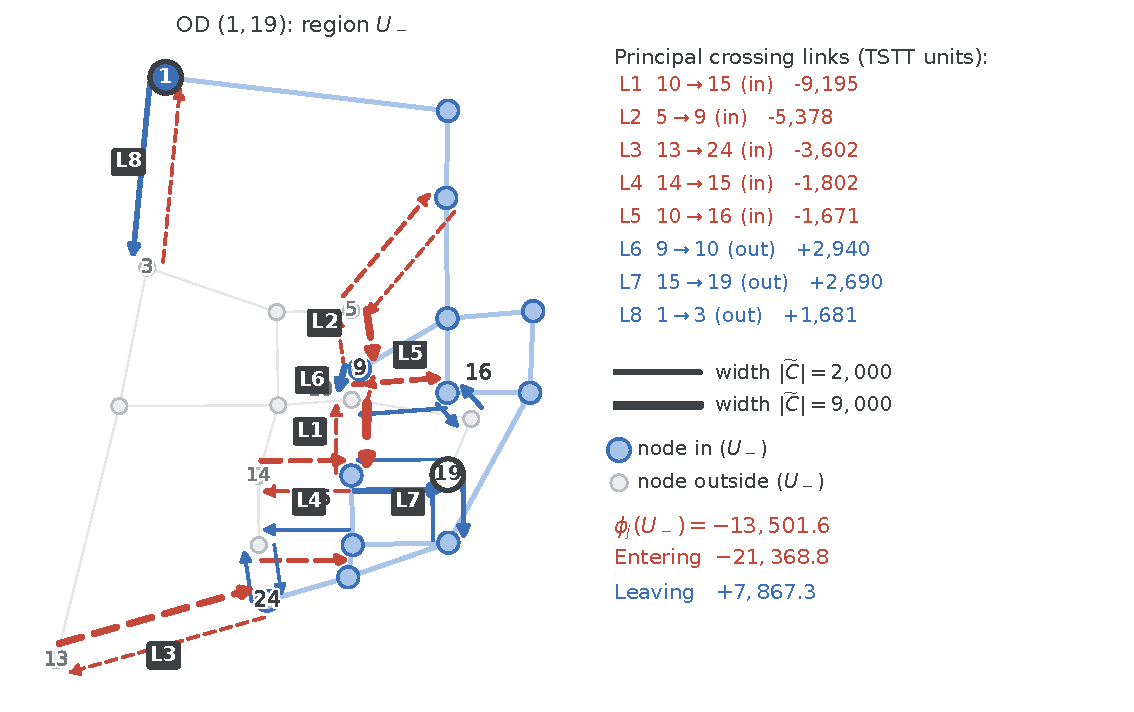
\includegraphics[width=0.82\linewidth]{../figures/fig_negmech_v102.pdf}
\caption{The connected minimizing region $U_-$ for OD $(1,19)$
(setting C, six-query protocol). Shaded nodes form $U_-$ (origin
node $1$ ringed; destination $19$ outside). Crossing-link arrows keep
the link direction; width scales with $|\widetilde C_{e,j}|$, and
colour and style encode the signed contribution to $\phi_j(U_-)$,
$a_{e,j}=\sigma_e\widetilde C_{e,j}$ ($\sigma_e=+1$ leaving, $-1$
entering; solid blue positive, dashed red negative), so a positive
attribution on an entering link appears red. The side panel lists, in
TSTT units, the five largest negative and three largest positive
contributions among the $26$ crossing links
($\mathrm{L}1$--$\mathrm{L}5$ negative, $\mathrm{L}6$--$\mathrm{L}8$
positive, ``(in)''/``(out)'' marking entering and leaving links),
with the width scale and the membership legend.}
\label{fig:negmech}
\end{figure}
\textbf{Endpoint identity checks.}
Appendix~\ref{supp:accuracy} reports the per-edge
endpoint-identity errors and their relation to completeness gaps on
these same demand paths.

\FloatBarrier
\subsection{Baseline surrogate envelopes}\label{supp:baselineenvelopes}
\begin{table}[pos=htbp]
\caption{Full-background surrogate validation on the identical
$41$-state path of the six-query protocol (setting C; TSTT units;
contributions and extrema rounded to integers, errors to one
decimal). $C_j^{\mathrm{learned}}$ and the connected extrema:
across-seed envelopes of per-model values (direct-SUE values in
Table~\ref{tab:newod}). Last two columns: five-seed
\emph{median} of the largest connected-boundary disagreement
$\epsilon_j^{\mathrm{cut}}$, in absolute units and as a percentage of
the direct connected span.}
\label{tab:fullbgsurrogate}
\footnotesize
\begin{tabular*}{\tblwidth}{@{\extracolsep{\fill}}lrrrrr}
\toprule
& & \multicolumn{2}{c}{Connected extrema: across-seed ranges}\\
\cmidrule(lr){3-4}
OD & $C_j$: across-seed envelope & per-model minima & per-model maxima & $\epsilon^{\mathrm{cut}}$ (med.) & $\epsilon^{\mathrm{cut}}$/span (med., \%)\\
\midrule
$(7,18)$ & $[574,\ 681]$ & $[335,\ 521]$ & $[907,\ 1{,}299]$ & $397.5$ & $522.5$ \\
$(1,19)$ & $[49{,}929,\ 51{,}452]$ & $[-13{,}911,\ -13{,}334]$ & $[23{,}683,\ 23{,}948]$ & $1{,}567.4$ & $4.2$ \\
$(4,5)$ & $[2{,}535,\ 2{,}934]$ & $[1{,}654,\ 2{,}148]$ & $[2{,}946,\ 3{,}546]$ & $1{,}050.8$ & $99.5$ \\
$(1,15)$ & $[77{,}416,\ 80{,}233]$ & $[-7{,}717,\ -6{,}766]$ & $[39{,}473,\ 40{,}076]$ & $2{,}187.3$ & $4.5$ \\
$(6,8)$ & $[73{,}565,\ 75{,}224]$ & $[36{,}412,\ 37{,}631]$ & $[66{,}892,\ 67{,}762]$ & $2{,}163.2$ & $6.9$ \\
$(7,12)$ & $[116{,}562,\ 118{,}706]$ & $[-17{,}084,\ -15{,}198]$ & $[59{,}965,\ 61{,}169]$ & $4{,}111.3$ & $5.3$ \\
\bottomrule
\end{tabular*}
\end{table}



\subsection{Fixed-screenline surrogate comparisons}\label{supp:screenlinelearned}
\begin{table}[pos=htbp]
\caption{Fixed straight screenlines: reference minimum and the five frozen flow-supervised surrogates at that same screenline (TSTT units). The last column gives the largest error over the screenline family, as an across-seed range.}
\label{tab:screenlinelearned}
\small\begin{tabular*}{\tblwidth}{@{\extracolsep{\fill}}lrrr}\toprule
OD & Reference minimum & Learned account: seed range & Maximum screenline error: seed range\\\midrule
$(7,18)$ & 642.4 & $[576.9,\ 789.8]$ & $[141.0,\ 269.4]$ \\
$(1,19)$ & -2766.6 & $[-3886.6,\ -3365.1]$ & $[857.9,\ 1430.8]$ \\
$(4,5)$ & 2652.3 & $[2301.7,\ 2918.8]$ & $[438.0,\ 648.3]$ \\
$(1,15)$ & 511.1 & $[732.8,\ 2068.2]$ & $[1140.6,\ 2553.0]$ \\
$(6,8)$ & 45230.2 & $[46431.5,\ 47218.3]$ & $[1276.2,\ 1988.1]$ \\
$(7,12)$ & -2967.3 & $[-2810.4,\ -1916.6]$ & $[1736.8,\ 2499.2]$ \\
\bottomrule\end{tabular*}\end{table}


\paragraph{Sign preservation.}\label{subsec:precision}
All five baseline seeds retain the three connected-family sign crossings
and positive system contributions. At the fixed reference extrema,
$m_j=\min\{-\phi_j^S(U_-),\phi_j^S(U_+)\}-\epsilon_j^{\rm conn}$
is positive, with smallest value 5519 TSTT units. This verifies sign
preservation without implying accurate column magnitudes.

At the fixed direct-model minimizing screenline, every baseline seed
retains the negative sign for both queries: $(1,19)$ gives
$[-3886.6,-3365.1]$ against the reference $-2766.6$, and $(7,12)$
gives $[-2810.4,-1916.6]$ against $-2967.3$. Their largest family-wide
errors across seeds are $1430.8$ and $2499.2$, below the respective
reference sign margins. These are screenline-specific certificates;
they supplement the separate connected-family result above
(Appendix~\ref{supp:screenlinelearned}).


The eight-query path-set and dispersion checks are collected in
Appendix~\ref{supp:coverage}. Boundary variation persists, although
the specified $(10,16)$ comparison $\{10\}\to\{10,17\}$ changes sign
across $\theta$; these are different fixed-path models, not convergence
to unrestricted SUE.
